% !TeX root = OptCuts.tex

\section{Coupled Discrete-Continuous Descent}
\label{sec:topologySearch}
To perform our primal update, we seek to minimize the Lagrangian over both continuous changes in vertex positions \emph{and} discrete changes in topology. 
%
To optimize over topology we could potentially perform exhaustive search over the graph of all possible mesh changes. This approach, however, is intractable for any practical mesh size. 
%
Instead, we devise a local search algorithm for topological updates inspired by the standard descent process of optimizing a smooth energy over vertex positions. 

%
%Instead, we begin by recalling the standard process of optimizing a smooth energy solely over vertex DoFs. In such cases, each iterate generally forms a localized approximation of the minimized energy \justin{didn't understand previous phrase} and then uses it to propose a candidate direction for decrease. Then, since finding such a direction is expensive, we search along the proposed direction to ensure a significant decrease in energy (and not increase). 
The descent standard process is to formulate a local approximation to the energy function, use it to estimate the direction for the gradient descent step, and then search along the proposed direction to find the step magnitude that ensures significant decrease in energy. 
%
We extend this process to include search over discrete variations in topology. In analogy to seeking a continuous search direction, at the start of each new primal solve we will build many localized energy approximations to search for a likely candidate mesh operation to repeatedly propagate topology change, i.e., cutting or merging, over our UV mesh. Each inner iterate of the primal solve will successively apply this operation in combination with standard smooth descent to explore discrete-continuous descent until no further progress is made.% and so a primal update is found.    %<-- doesn't seem needed

In the remainder of this section we formulate the energy model that is used to evaluate the candidate topology operations (Section ~\ref{sec:topology_energy}), 
enumerate the topology operations used in our algorithm (Section~\ref{sec:topology_ops}), explain how we find the search direction (Section~\ref{sec:descent_op}), and iteratively explore the identified direction (Section~\ref{sec:topology_search}).

\subsection{Energy Model for Topology Updates}
\label{sec:topology_energy}
We next devise an approximate energy model to efficiently estimate the effect of a potential topological change. 
To keep our notation simplified, in the following we use $i$ or $j$ to index the inner loop of the primal update and $k$ for indexing the outer loop.
At each outer iterate $k$, the optimal Lagrangian for any proposed topology $T^i$ is  
\begin{align}
\ell(T^i) = \min_{U} L(T^i, U) = E_s(T^i) + \lambda^k \min_{U} E_d(T^i, U).
\end{align}
Then, for any valid topology-changing operation, $o^{i,j}:T^i \rightarrow T^j$, the resultant change in Lagrangian is $\Delta \ell(o^{i,j}) = \ell(T^j) - \ell(T^i)$. We seek a valid operation that will produce large decrease in the Lagrangian.


Since minimizing over $U$ for every potential topology change is intractable for large meshes, we start from a known $(T^i, U^i)$, and approximate the change in the Lagrangian by restricting the distortion update to the locally changed vertex stencil $U^{i,j}$ of the applied topological operation $o^{i,j}$. We choose the stencil to include only the vertices affected by the topological operation and their immediate neighbors.
We hold all other vertices $U_s$, shared in common with $T^i$, fixed in the mesh
to the same positions previously held in $U^i$, so that vertex positions after the update are $U^j = (U^{i,j}, U_s)$.  Our approximate change in Lagrangian is then 
%\danny{TODO: Still need some syntatic sugar to make this decomposition of fixed and free new vertices clean.}
\begin{align} 
d(o^{i,j}) = E_s(T^i) + \lambda^k \min_{U^{i,j}} E_d \big( T^i, (U^{i,j}, U_s) \big) - L(T^i,U^i,\lambda^k).
\end{align}
%
Evaluating $d$ requires solving continuous distortion optimization with respect to stencil vertices $U^{i,j}$. We use Newton-type smooth descent for this; see Section~\ref{sec:descentStep} for details.

\subsection{Local Topological Operations}
\label{sec:topology_ops}

We consider descent with topology changes induced by three mesh operations.

\paragraph{Boundary Vertex Split}
Boundary vertices can be split along any interior incident edges. 
Each such candidate split generates two duplicate vertices forming the stencil to compute $d$.
\begin{wrapfigure}[5]{r}{0.4\linewidth}
  \begin{center}
  \vspace{-4mm}
    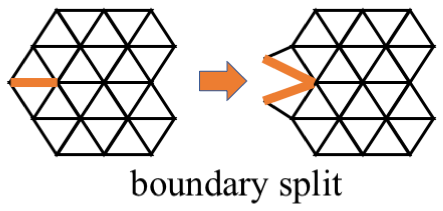
\includegraphics[width=1\linewidth]{fig/bSplit}
  \end{center}
\end{wrapfigure}
When splitting a boundary vertex along an edge connecting to another boundary vertex, we either remove a hole or else produce a new chart in our UV map. For the latter case, we generate four duplicate vertices forming the stencil to compute $d$.
%\minchen{[TODO] 4-vertex merge to support joining two charts together, triangle moving operations?}

\paragraph{Interior Vertex Split}
\begin{wrapfigure}[4]{r}{0.4\linewidth}
  \begin{center}
  \vspace{-4mm}
    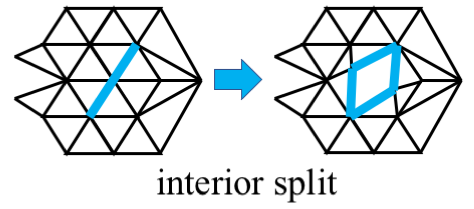
\includegraphics[width=1\linewidth]{fig/iSplit}
  \vspace{-1mm}
  \end{center}
\end{wrapfigure}
Interior vertices can be split along 
any pair of incident edges. Each such candidate split generates two duplicate vertices forming the stencil to compute $d$. 
%We ignore potential interior splits when this would be connected to an existing seam, as this is overloaded with propagating the boundary vertex split operation.

\paragraph{Corner Merge}
Corners are formed by three UV vertices corresponding to the tail edge of a cut seam on the input surface. 
\begin{wrapfigure}[5]{r}{0.4\linewidth}
  \begin{center}
  \vspace{-5mm}
    \includegraphics[width=1\linewidth]{fig/cMerge}
  \vspace{-4mm}
  \end{center}
\end{wrapfigure}
Merging the end vertices generates a single new vertex forming the stencil to compute $d$. Merging requires extra care here. Unlike vertex splitting, an initial location for the newly merged vertex must be selected. Na\"ive merging can violate local injectivity and so prevent progress if we are working with barrier-type energies like symmetric Dirichlet. We initialize a merged vertex to the average of its parent vertices. If inversion is detected, we then apply Agmon's relaxation~\shortcite{Agmon1954Relaxation} to project to an inversion-free position iteratively. On rare occasions this will not suffice and so we remove the proposed operation from our queue.
%However, cases are still there when only moving the merged vertex is not enough to obtain an inversion free initial local stencil. In these situations, we will just abandon the candidate. This rarely happens in practice and does not affect our result.\justin{didn't follow the last two sentences, maybe needs a small figure}

\subsection{Topology Search Candidates}
\label{sec:descent_op}
In analogy to computing a continuous search direction, at the start of each new primal solve we search for a candidate mesh operation to propagate descent. 
%
We first consider boundary vertex splits originating at one of $m$ boundary vertices in the current topology $T^k$. 
To reduce unnecessary computational overhead we select a subset of $m_\text{boundary}=m^{0.8}$ boundary vertices that might have the largest effect on the energy. To estimate the priority, we compute the standard deviation over all the distortion energy gradients acting on the boundary vertex contributed from incident elements. We then pick boundary vertices with largest deviation, i.e. where distortion might best be alleviated by cutting. We use the selected vertices to initiate boundary vertex splits, and consider all current seams for a corner merge, building a set $O^k$ of potential topological operations.
%
%We use the selected vertices to build a set of candidate mesh operations $O^k$ formed by boundary vertex splits and all valid corner merges on those vertices. 
We then find a minimizer for the first topological change:
\begin{align}
\label{eq:minO}
o^{0,1} = \argmin_{o \in O^k} d(o).
\end{align}
Since we use local support for vertex stencils, all queried $d$ in this minimization can be efficiently evaluated in parallel. 

It is possible for none of the boundary cuts to yield a decrease in energy (i.e., $d(o^{0,1}) \geq 0$).  In this case, we consider initiating a new seam via an interior vertex split. In a similar process, we then pick $m_\text{interior}=(n-m)^{0.8}$ interior vertices with the largest deviation of distortion energy gradients, and build  $O^k$ as the set of all interior vertex splits on those vertices. We select the $d$-minimizing interior split operation $o^{0,1} \in O^k$ using (\ref{eq:minO}). Once we identify the best topological change $o^{0,1}$, i.e.\ our search direction, we next expand it via iterative propagation. 

%After estimating the minm $o^{i,j}$
%
%we set our candidate mesh operation for our descent process, $s^k$, with this operation, $s^k \leftarrow o^{i,j}$. Otherwise, we initiate new seams via interior vertex splits. Similarly to before, we pick $m_\text{int}=(n-m)^{0.8}$ interior vertices with the largest deviation, and build  $O^k$ as the set of all interior vertex splits on those vertices. We select the $d$-minimizing interior split operation $o^{i,j} \in O^k$, again using (\ref{eq:minO}), is then set as the set $s^k \leftarrow o^{i,j}$ for our descent process.

\subsection{Iterated Search, Propagation and Descent}
\label{sec:topology_search}

We propagate the best seed topological operation $o^{0,1}$ by iteratively applying operations of the same type (a boundary or interior split, or a merge). During the primal update we alternate between propagating topological change, updating $T^i$, and a smooth coordinate update on $U^i$.

%Once we have computed our candidate search operation $s^k$, we begin an inner loop iteration, indexed by superscript $i$ (recalling outer iterates are indexed by $k$), to solve the primal variable update. 

%At the start of this process we initialize our desired upper bound on estimated decrease to $\delta^0 = 0$; this will be updated at each successive iterate. 
%Then, each inner iteration $i$ proceeds by first propagating topology change followed by smooth coordinate update. 

Each topology propagation step first generates a set of all possible mesh operations $\mathcal{E}(o^{i-1, i}, T^{i})$ that could continue to propagate the previous operation $o^{i-1, i}$ on the current topology $T^{i}$; e.g., all valid edges to extend an existing seam at its tail. Figure~\ref{fig:propagation} illustrates how we propagate each type of topological operation.
%
Here we then pick a $d$-minimizing operation from this small set of candidate operations for our next operation to apply,
\begin{align}
\label{eq:minE}
o^{i,i+1} = \argmin_{o \in \mathcal{E}(o^{i-1, i}, T^i)} d(o).
\end{align}

Since each change in topology alternates with smooth coordinate descent and we wish to come close to a local minimized of distortion in each primal solve, we work to avoid introducing too many topological changes as long as the coordinate update provides significant energy improvement. We denote the threshold for desired estimated decrease by $\delta^{i}$. It is initialized to $\delta^0=0$ in the first iteration, and then set to the distortion energy improvement from each successive coordinate update. At any iteration, if $d(o^{i,i+1}) < \delta^{i}$ we update the topology based on the best operation $T^{i+1} \leftarrow o^{i, i+1}(T^{i})$ and keep it unchanged otherwise, $T^{i+1} \leftarrow T^i$.

%If this minimizer provides sufficient estimated decrease, so that $d(o^{i,i+1}) < \delta^{i}$, we accept the topology update setting $T^{i+1} \leftarrow o^{i, i+1}(T^{i})$; otherwise, we keep topology unchanged with $T^{i+1} \leftarrow T^i.$

\begin{figure}[t]
\centering
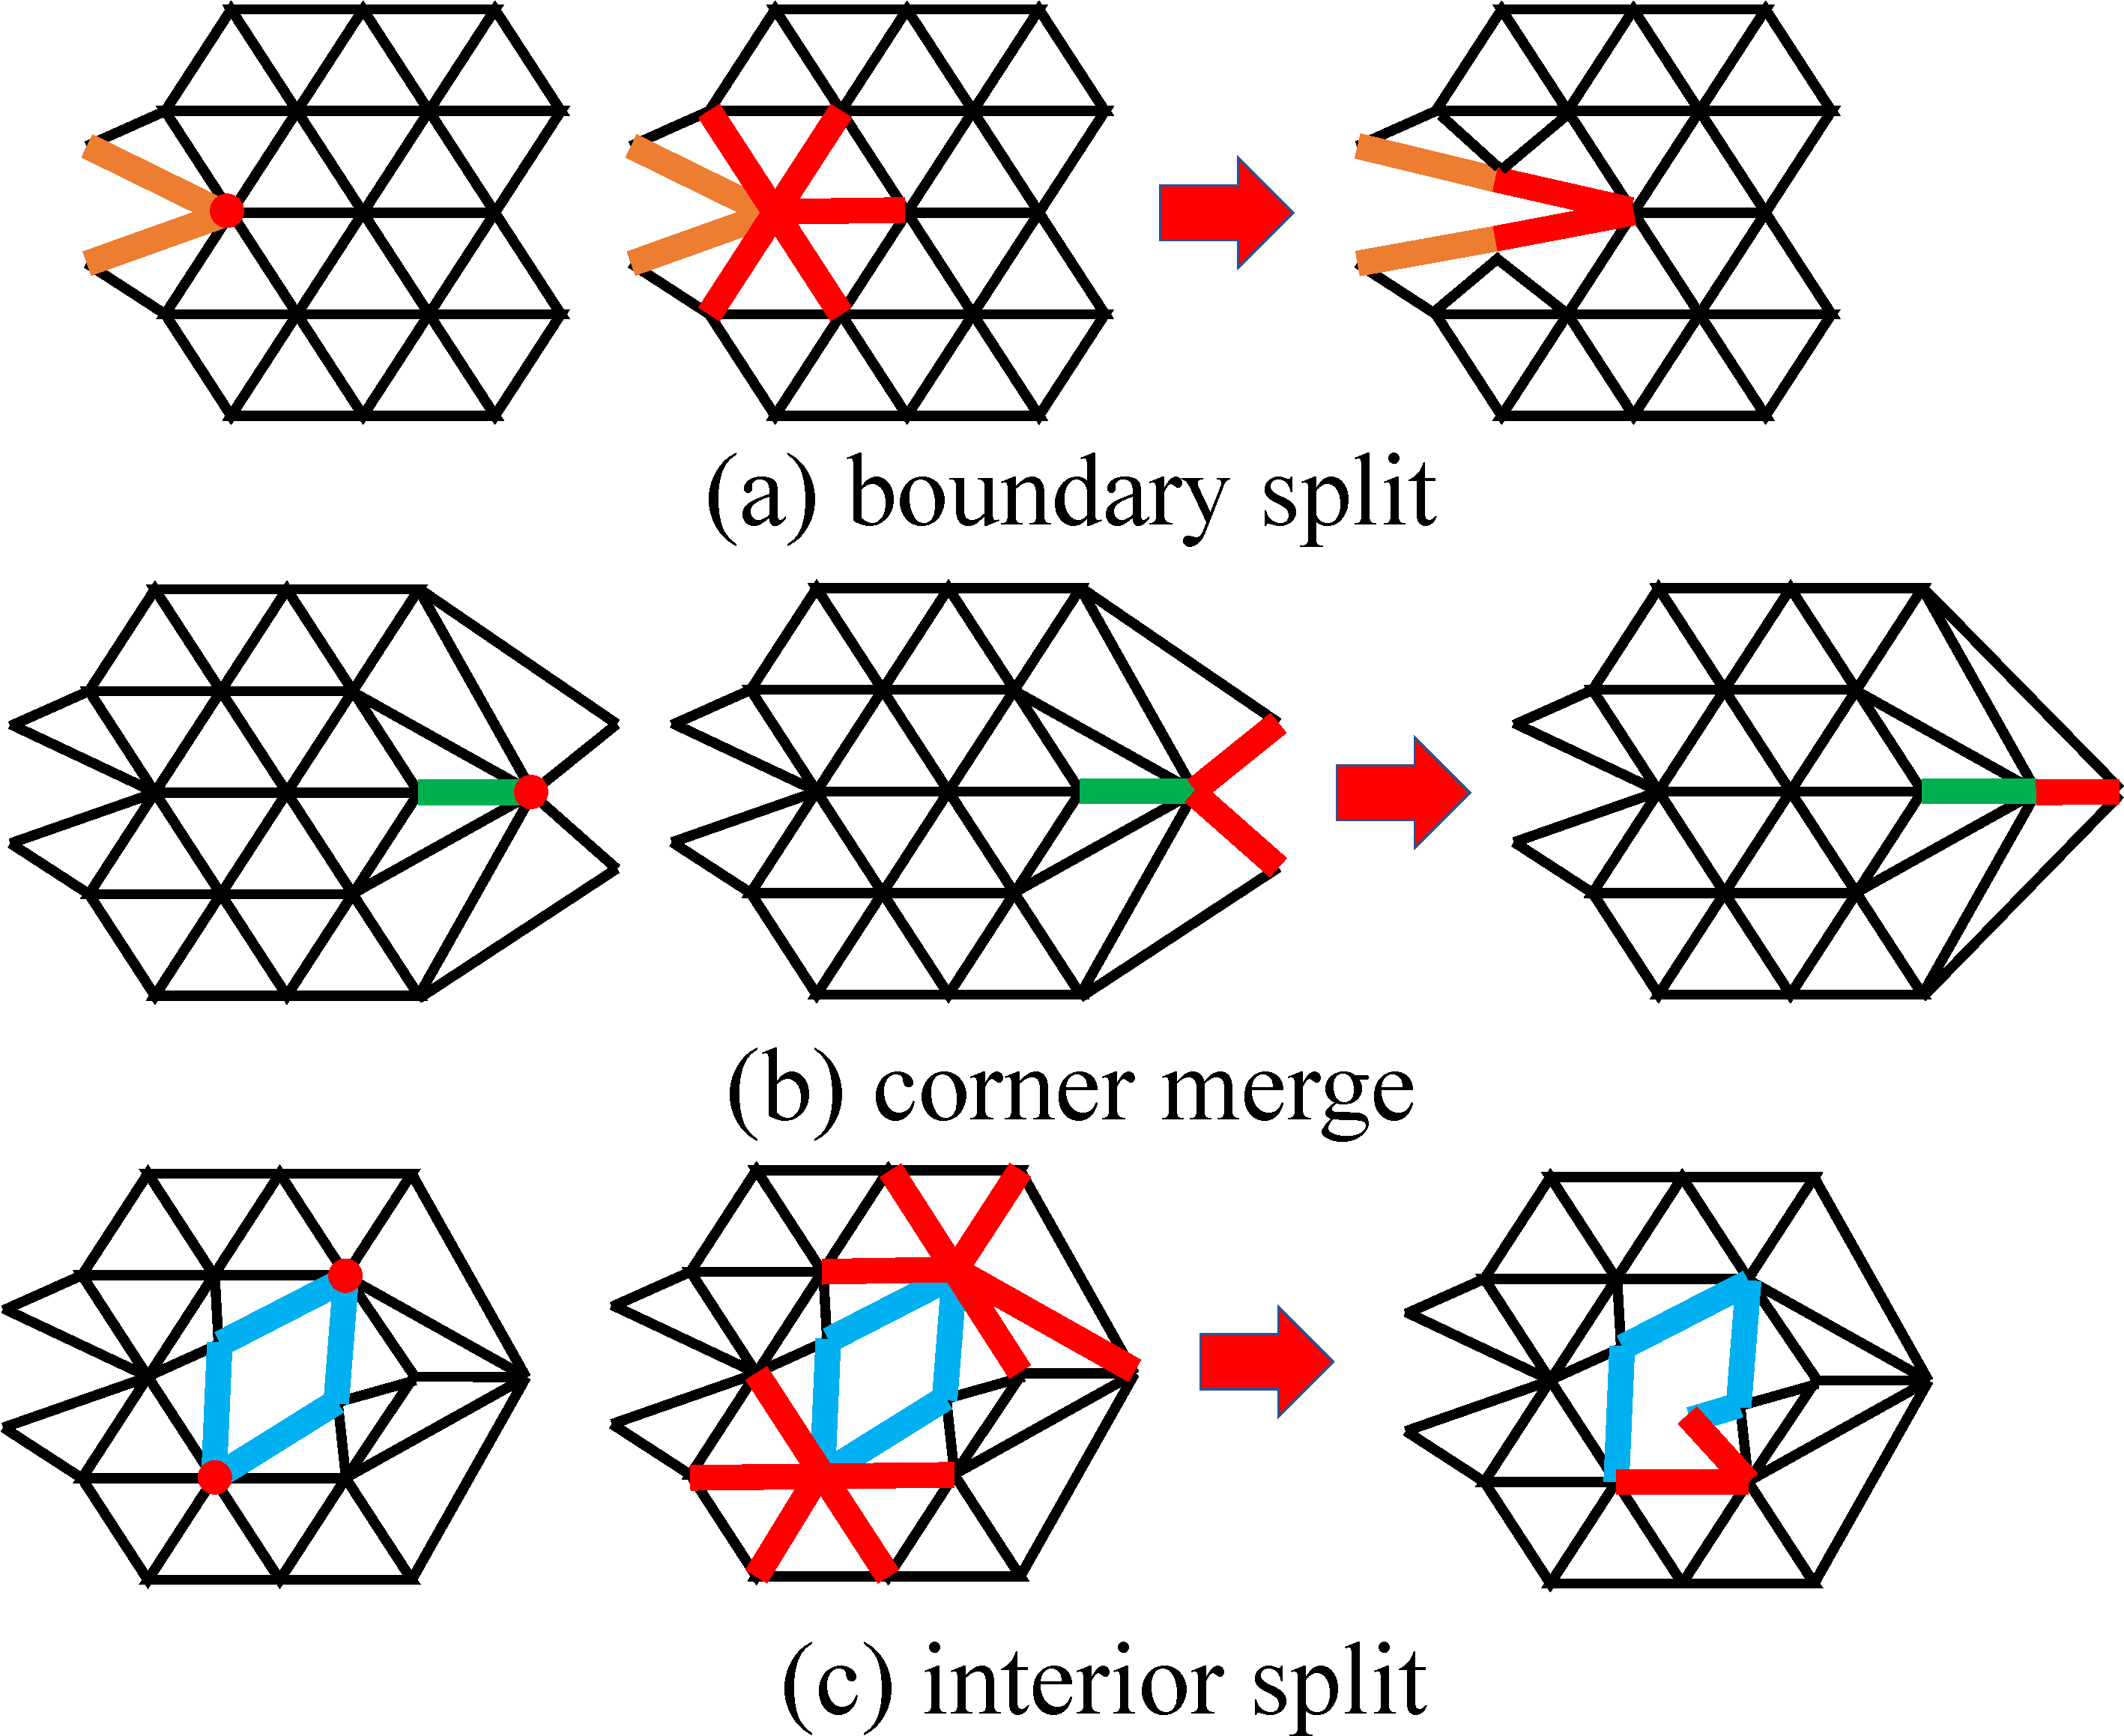
\includegraphics[width=0.65\linewidth]{fig/propagation.pdf}
\caption{Propagation of boundary split (orange), corner merge (green), and interior split (blue). When a propagating boundary split, all edges that could continue to propagate a boundary splitting cut from the current tail would be considered (a); for corner merge we just query the new corner at the current tail (b); for an interior split, once an incident edge of either the two tail is split as propagation, in the following iterations it would be the same as propagating boundary split (c).}
\label{fig:propagation}
\end{figure}

The subsequent coordinate update then simply applies a single step of projected Newton descent with line search to update the vertex coordinates $U^i$; see Section~\ref{sec:descentStep} for details. We then ask for the next topology update to gain similar or greater magnitude decrease by setting $\delta^i = E_d(U^i) - E_d(U^{i-1})$.

This process terminates at iteration $i+1$ when smooth iterations have converged (see Section~\ref{sec:descentStep} on varying conditions for this) \emph{and} the propagation of the seed mesh operation produces no further descent. We then set $(T^k,U^k) \leftarrow (T^{i+1},U^{i+1})$ and begin the next outer iterate $k+1$ with the dual variable update. 


